The best result are the one performed by \textit{K-Means}: the feature are extracted with \textit{Standardization}, \textit{Normalization} and \textit{PCA} with my custom feature subset implementation, the number of cluster given as input is estimated through the \textit{Elbow method} from \textit{WCSS} graph, and the results are given in terms of plot representation and \textit{Silhouette score}. 

In particular the feature extraction phase has been performed with different features configuration. The best result is produced with my custom implementation of PCA on the following subset of features: 

\begin{align}
\{ &\{ latitude\} , \{longitude\}, \notag\\
 &\{spread\-latitude, spread\-longitude\}, \notag\\
 &\{edge\-latitude\-start, edge\-latitude\-stop, \notag\\ 
 &\phantom{\{}edge\-longitude\-start, edge\-longitude\-stop\} \}\notag
\end{align} 

But it doesn't perform result widely better than the traditional PCA approach based on the $80\%$ of cumulative variance. Moreover, feature extraction without time features produces better clustering result. Time is a feature dimension that brings cluster algorithms to a worse prediction, because the same trajectory could be travelled in different time and instead I want to find the common trajectory independently by time. On the other hand, time is very useful to find subgroups of the same trajectory, as performed by \textit{timedelta heuristic}.

Moreover I tried to compare \textit{K-Means} clustering with and without PCA. The figure \ref{fig:kmeans-without-pca} shows \textit{K-Means} clustering algorithm performed without PCA on latitude and longitude features only. This comparison shows how PCA improve the variance on clustering prediction, and the presence of heuristic features maintains the rental division, on which the heuristic algorithms has been executed.  

\begin{figure}[bt]
	\centering
	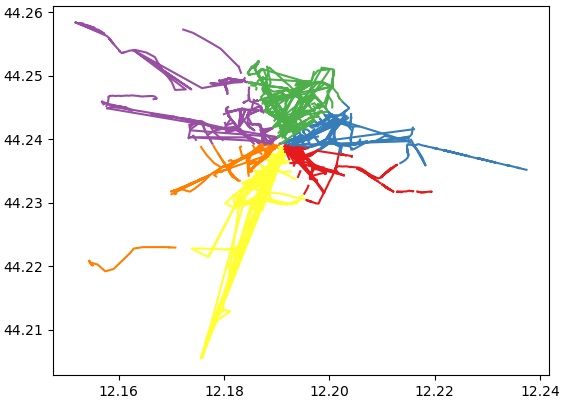
\includegraphics[width=\columnwidth]{kmeans-without-pca}
	\caption{K-Means without PCA with only latitude and longitude features}
	\label{fig:kmeans-without-pca}
\end{figure}

The tests performed shows how difficult is the clustering operation on trajectories very distant from each other. In fact, the positions of this dataset involves mainly in two Italy cities and performing a clustering algorithm on both, it will try to create 2 clusters. Since I would like to obtain more cluster, in order to group trajectory inside the cities, I tried to increment the number of clusters. A \textit{K-Means} clustering execution on the whole positions with 5 clusters performs really bad results (figure \ref{fig:kmeans-bad}). Therefore, clustering has always to be performed on a specific region of interest in order to optimize the results.

\begin{figure}[bt]
	\centering
	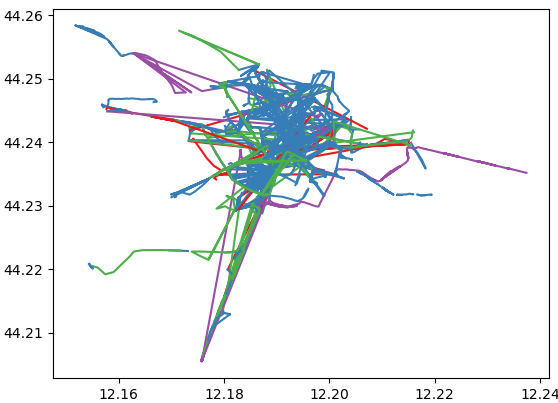
\includegraphics[width=\columnwidth]{kmeans-bad}
	\caption{K-Means with 5 clusters, PCA, Standardization and Normalization performed on all positions showed on one city}
	\label{fig:kmeans-bad}
\end{figure}

Lastly, I noticed that \textit{silhouette score} is never higher than $0.5$, while its maximum value could arrive to $1.0$. This score could indicate that the result is not very good, but actually \textit{silhouette score} is not an validation methodology so reliable, because it depends a lot on the data you are dealing with. In particular, \textit{silhouette validation} uses a distance metric to produce this value, therefore it will be very reliable when used for circular shape clustering (in 2D) but for other type of distribution, you shouldn't give it too much importance, but rather consider a visual representation of results. In our case, trajectories will hardly have a circular shape, consequently a positive means silhouette score of $0.3$ is pretty good for this kind of clustering.

For sure, \textit{edgedelta} and \textit{coorddelta} heuristic can be improved, and more advanced clustering techniques can be implemented in order to obtain better results. 